\chapter{Evaluation}
\label{chap:evaluation}
In this chapter we aim to evaluate different aspects of the developed system. This includes a cost analysis, a performance analysis and finally a field test of a simplified artwork tracking scenario.

\section{Cost and Performance Analysis}
The primary cost factor of the artis-system is the \gls{sc}. Each execution of a function that mutates the state of the \gls{sc} costs a certain amount of gas which in turn has a price in Ether. A transaction thus is calculated as follows:
$$
transaction\ fee = gas \times gas\ price
$$
To analyze the execution costs of the \textit{safeMint} and \textit{updateArtworkData} contract functions, we executed the corresponding requests of the developed \gls{api} multiple times $(n = 10)$ and recorded transaction fees as well as the request time in seconds. This analysis was conducted on the sepolia testnet and the resulting transactions were inspected on the Etherscan block explorer. To execute and time the \gls{http} requests we used Postman \cite{postman}.

\begin{figure}[h!]
    %\centering
    \begin{subfigure}{0.5\textwidth}
        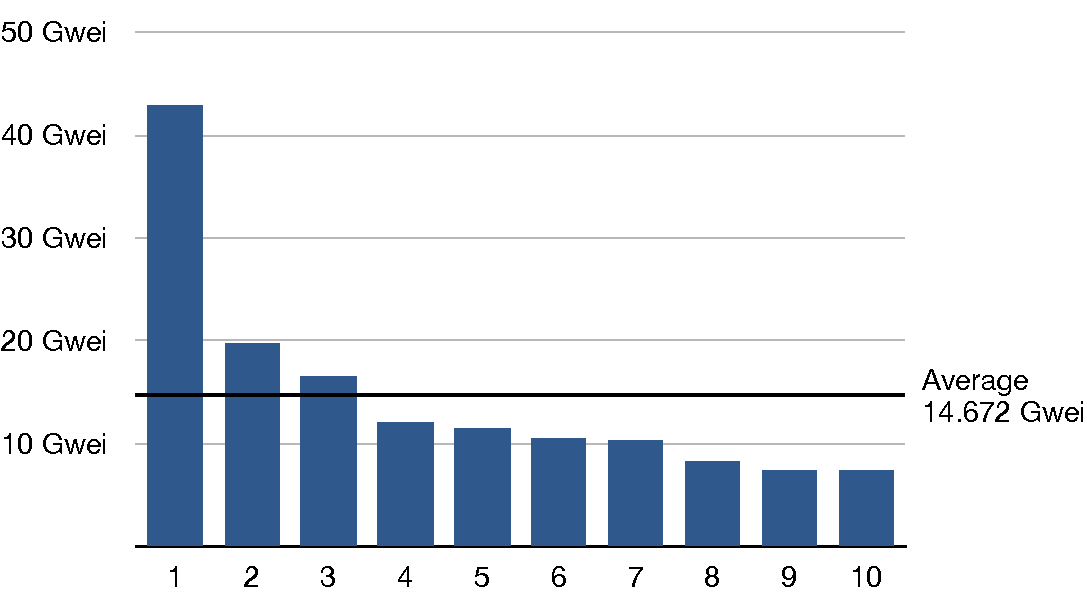
\includegraphics[width=\textwidth]{diagrams/safeMint_tx_cost.pdf}
        \caption{Transaction cost in Gwei}
        \label{fig:safemint_tx_cost}
    \end{subfigure}
    \hfill
    \begin{subfigure}{0.5\textwidth}
        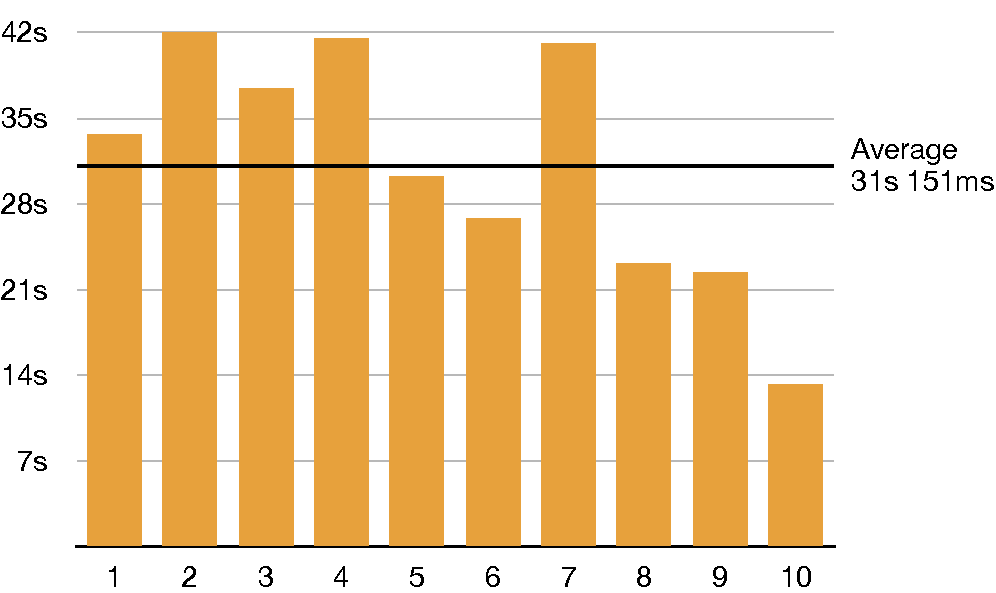
\includegraphics[width=\textwidth]{diagrams/safeMint_tx_speed.pdf}
        \caption{Request speed in seconds}
        \label{fig:safemint_tx_speed}
    \end{subfigure}
    \caption{SafeMint analysis}
    \label{fig:safemint_analysis}
\end{figure}

\subsection*{safeMint}
As visualized in Figure \ref{fig:safemint_analysis} the transaction fees, on average, amount to 14.7 Gwei. At the time of writing (August 8, 2023), the price for one Ether is 1'843.58 \gls{usd} \cite{coinmarketcap}. This means on average it would cost arount $0.000027$ \gls{usd} to create a new artwork \gls{nft}, or in other words around 36'000 \glspl{nft} per \gls{usd}.

The average time to fulfill such a request is around $31$ Seconds. As shown in Figure \ref{fig:safemint_tx_speed}, the time varies and ranges from less than $14$ Seconds to around $42$ Seconds.

\subsection*{updateArtworkData}

\subsection*{Non-Mutating Functions}
The GET endpoints exposed by the \gls{api} target several functions that do not mutate the state of the \gls{sc}. These functions do not cost any gas and their execution time is much less (usually < 1 Second). Additionally, the artis-server adds a caching layer to these function calls which generally reduce the response time of repeated calls to a few milliseconds. 

\section{Field Test}
In addition to the above analyses, we also performed a simulated scenario of transporting an artwork. This test is composed of several steps:

\begin{enumerate}
    \item create a new artwork \gls{nft} and register the corresponding roles using the artis-frontend.
    \item request the status of the artwork to be changed to \textit{IN\_TRANSIT} from the sender account
    \item approve this request from the carrier account
    \item enable the logger by starting the \textit{logging\_script} and the \textit{violation\_script} with the thresholds of 27 degrees Celcius and 70\% humidity.
    \item take the logging device and transport it from point of departure to destination
    \item during the transportation simulate a violation by wrapping a hand around the sensor to increase the temperature.
    \item upon arrival request the status of the artwork to be changed to \textit{DELIVERED} from the carrier account
    \item approve this request from the recipient account
\end{enumerate}

%section discussion